%%%%%%%%%%%%%%%%%%%%%%%%%%%%%%%%%
% Laatste aanpassing:           %
% 6 sept 2013 [Jan]: kleine aanpassingen
% 28/06/13 [Greetje]: Verbeterd en examenvragen van Leentje toegevoegd
% 23/3/11 [Greetje]: Volledig herwerkt
%
% 10/09/01 door Greetje
%   verbeteringen van Roos
%   rekenregels weggelaten
%
% 01/09/01 door Greetje          %
%%%%%%%%%%%%%%%%%%%%%%%%%%%%%%%%%

\section{Oefeningen}
\begin{oef}     
Los de volgende vergelijkingen op naar $x$. 
\begin{multicols}{2}
\begin{enumerate}
  \item $3^{-x+2}=0,7^{2\cdot x}$
  \item $4^{x}-5\cdot 2^{x}-24=0$
  \item $3^{x}+3^{x+1}=4$
  \item $3^{x+1}-26=3\cdot 3^{-x}$
  \item $2^{3^x}=8$
  \item $9^{x+1}-2\cdot 3^{x+2}-27=0$
  \item $5^{x+1}=5^{3x+1}$
  \item $2^{x+3}=16^{x-3}$
  \item $3^x=59049$
  \item $\left(\frac12\right)^x=2048$
  \item $7^x=2\cdot 8^x$
  \item $2^{x+3}=16^{x-3}$
  \item $100 \cdot 1,05^x=2000\cdot 1,025^x$
  \item $15\cdot 3^{x+1}-243\cdot 5^{x-2}=0$
  \item $3^{4x+5}=5^{x-1}$
  \item $5^{(2^x)} = 25^{(8^x)}$
\end{enumerate}
\end{multicols}
\begin{opl}
\begin{enumerate}
  \item \[
          \begin{array}{rrclcl}
                 & 3^{-x+2} & = & 0.7^{2x} \\
            \iff & 9 \cdot 3^-x & = & 0.7^{2x} \\
            \iff & 9 & = & 0.7^{2x} \cdot 3^x \\
            \iff & 9 & = & (0.7^2 \cdot 3)^x \\
            \iff & \log(9) & = & x \log(0.7^2 \cdot 3) \\
            \iff & x & = & \frac{\log(9)}{\log(0.7^2 \cdot 3)} & \approx & 5.70319
          \end{array}
        \]
  \item \[
          \begin{array}{rrclcl}
                 & 4^x - 5 \cdot 2^x - 24 = 0
            \iff & (2^x)^2 - 5 \cdot 2^x - 24 = 0
          \end{array}
        \]
        We voeren $z = 2^x$ in, dit geeft ons
        \[
          z^2 - 5z - 24 = 0
        \]
        Dit is een vierkantsvergelijking met als discriminant
        \[
          D = (-5)^2 - 4 \cdot 1 \cdot (-24) = 25 + 4 \cdot 24 = 121
        \]
        en met twee oplossingen
        \[
          z_1 = \frac{5 - \sqrt{D}}{2} = -3 \qquad z_2 = \frac{5+\sqrt{D}}{2} = 8
        \]
        Dit geeft ons
        \[
          2^{x_1} = -3 \qquad 2^{x_2} = 8
        \]
        De linkervergelijking heeft geen oplossing, de rechter heeft als oplossing $x_2 = \log_2(8) = 3$.
  \item \[
          \begin{array}{rrclcl}
                 & 3^x+3^{x+1} & = & 4 \\
            \iff & 3^x+3^x\cdot3 & = & 4 \\
            \iff & 3^x(1+3) & = & 4 \\
            \iff & 3^x & = & 1 \\
            \iff & x & = & 0
          \end{array}
        \]
  \item \[
          \begin{array}{rrclcl}
                 & 3^{x+1}-26 & = & 3 \cdot 3^{-x} \\
            \iff & 3^{2x+1}-26 \cdot 3^x & = & 3 \\
            \iff & 3 \cdot (3^x)^2-26 \cdot 3^x - 3 & = & 0 \\
          \end{array}
        \]
        Substitutie $z = 3^x$
        \[
          3 z^2 - 26 z - 3 = 0
        \]
        Dit is een vierkantsvergelijking met
        \[
          D = (-26)^2 - 4 \cdot 3 \cdot (-3) = 712
        \]
        en
        \[
          z_1 = \frac{26 - \sqrt{D}}{6} \approx -0.11 \qquad z_2 = \frac{26 + \sqrt{D}}{6} \approx 8.78
        \]
        $z_1 = 3^x$ geeft ons geen oplossingen, maar
        \[
          \frac{26 + \sqrt{D}}{6} = 3^x \iff x = \log_3\left( \frac{26 + \sqrt{712}}{6} \right) \approx 1.98
        \]
  \item \[
          \begin{array}{rrclcl}
                 & 2^{(3^x)} & = & 8 \\
            \iff & 2^{(3^x)} & = & 2^3 \\
            \iff & 3^x & = & 3 \\
            \iff & x & = & 1
          \end{array}
        \]
  \item $9^{x+1} - 2\cdot 3^{x+2}-27=0$
        \[
          \begin{array}{rrclcl}
                 & 9^{x+1}-2 \cdot 3^{x+2}-27 & = & 0 \\
            \iff & 9 \cdot (3^x)^2 - 18 \cdot 3^x - 27 & = & 0
          \end{array}
        \]
        Substitutie $z = 3^x$
        \[
          9 z^2 - 18 z - 27 = 0
        \]
        Dit geeft een vierkantsvergelijking met
        \[
          D = (-18)^2 - 4 \cdot 9 \cdot (-27) = 1296 \qquad \sqrt{D} = 36
        \]
        en oplossingen
        \[
          z_1 = \frac{18 - 36}{18} = -1 \qquad z_2 = \frac{18 + 36}{18} = 3
        \]
        $z_1 = -1$ geeft geen oplossingen voor $x$, maar
        \[
          3 = 3^x \iff x = 1
        \]
  \item $5^{x+1}=5^{3x+1}$
  \item $2^{x+3}=16^{x-3}$
  \item $3^x=59049$
  \item $\left(\frac12\right)^x=2048$
  \item $7^x=2\cdot 8^x$
  \item $2^{x+3}=16^{x-3}$
  \item $100 \cdot 1,05^x=2000\cdot 1,025^x$
  \item $15\cdot 3^{x+1}-243\cdot 5^{x-2}=0$
  \item $3^{4x+5}=5^{x-1}$
  \item $5^{(2^x)} = 25^{(8^x)}$
\end{enumerate}
\end{opl}
\end{oef}

% Oefeningen op logaritmische vergelijkingen
%\begin{oef} $\qquad$
% \\
%\begin{multicols}{2}
%\begin{enumerate}
%\item   $3 \cdot \log_{2}2 +\log_{2}x=3$ 
%\\ \item   $\log_{x}(\sqrt{3})=3$
%\\ \item    $\log(2x+3)+\log(x-1)=\log(x^{2}+9)$
%\\ \item     $\log_{64}(\log_{x}(16))^{3}=1$ 
%\\ \item $(\log_{2}x)^{3}+\log_{2}(x^{4})=4\cdot (\log_{2}x)^{2}$
%\\ \item  $\displaystyle{\log_{2}x=\frac{1}{\log_{6-x}4}}$
%\\ \item $\log_{2}(2^{x}-7)+x=3$
%\\ \item $\log_{x}(2\cdot x+8)=2$ 
%\\ \item $\log(x-3)+\log(x+1)=\log(2x+2)$
%\\ \item  $\left[\log(x+2)\right]^3+\left[\log(x+2)\right]^2=\log\left[(x+2)^2\right]$
% \end{enumerate}
%    
%\end{multicols}
%
%     \end{oef}
     
\begin{oef}
  Een blad papier is 1 mm dik. We plooien dit blad een
     \emph{aantal keren na elkaar} dubbel. In de veronderstelling dat
     we dit proces heel dikwijls na elkaar \emph{kunnen} uitvoeren,
     hoeveel keren moeten we minstens plooien opdat de dikte van
     het geplooide blad papier meer dan 2 cm zou meten?
     \begin{opl}
     Dikte van geplooide papier: $D(t)=2^t$.\\
     Zoek $t$ zodat $D(t)=20$. Dit geeft $t=\log20/\log 2=4,32$.\\
     Antwoord: na vijf keer plooien is dikte meer dan 2 cm.
     \end{opl}
\end{oef}

\begin{oef}
 We nemen aan dat op korte termijn de waarde van een aandeel stijgt
      volgens een exponentieel  proces. Op 10 maanden is de prijs van
      het aandeel verdrievoudigd.
      \begin{enumerate}
          \item    Bepaal de groeifactor (i) per 10 maand en (ii) per maand van dit groeiproces.
          
	 \item  Als je weet dat het aandeel nu het vijfvoud is van
          toen het werd aangekocht, hoeveel maanden geleden is het dan
          aangekocht?
      \end{enumerate}
      \begin{opl}
      \begin{enumerate}
      \item $g_{10}=3$; $g_m=3^\frac{1}{10}$
      \item Waarde van aandeel in functie van de tijd: $B(t)=B(0)\cdot 3^\frac{t}{10}$ \\
      Zoek $t$ zodat $B(t)=5B(0)$. Dat geeft $t=\log5/\log3^\frac{1}{10}=14,65$, dus na 14,65 maanden.
      \end{enumerate}
      \end{opl}
       \end{oef}

 
  \begin{figure}[hbtp]
      \flushright
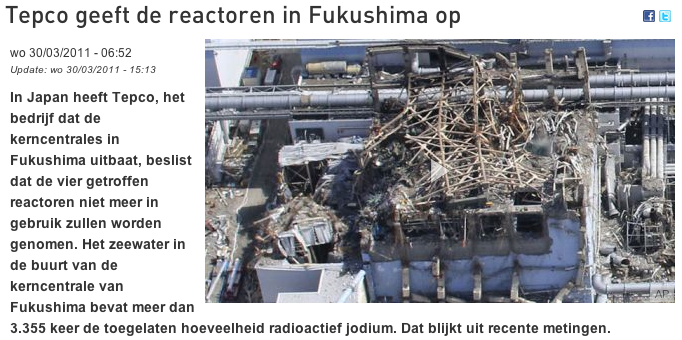
\includegraphics[width=0.95\textwidth]{oefeningen/jodiumderedactie.png}
\caption{Fukushima -- De redactie, 30 maart 2011}
\label{fig:fukushima} 
\end{figure}    
\begin{oef}
In 2011 werd Japan getroffen door een zware aardbeving met bijbehorende tsunami. De kernreactoren in Fukushima konden niet meer gekoeld worden en ontploften gedeeltelijk. Op 30 maart 2011 (figuur~\ref{fig:fukushima}) bleek de hoeveelheid radioactief Jodium in het zeewater ($\text{I}^{131}$) 3355 keer de toegelaten hoeveelheid te bedragen. 
De Japanse overheid beweerde dat er geen probleem was voor de consumptie van vis uit de zee, want de radioactiviteit zou snel verdund worden. Bereken hoelang het duurt (bij deze verontreiniging) tot de radioactiviteit van het $\text{I}^{131}$ terug gelijk is aan de toegelaten hoeveelheid. De halveringstijd van $\text{I}^{131}$ is 8 dagen.
      \begin{opl}
      $J(t)=3355\cdot J_0\cdot \left( \frac12\right)^\frac{t}{8}$\\
      Zoek $t$ zodat $J(t)=J_0$\\
      $t=8\frac{\log \frac{1}{3355}}{\log\frac12}=93,70$, dus na 93,70 dagen.
      \end{opl}
      \end{oef}


\begin{oef}
 Op een archeologische site werden muurschilderingen
    teruggevonden. De ouderdom van de schildering wordt bepaald
    met de $\text{C}^{14}$-proef.  Men weet immers  dat de
    hoeveelheid van dit isotoop jaarlijks exponentieel daalt met factor
    \num{0.99988}. Op de schilderingen werd \SI{20}{\percent} van de
    oorspronkelijke hoeveelheid $\text{C}^{14}$ teruggevonden. Hoe oud
    zijn de schilderingen?
    \begin{opl}
    $C(t)=0,20\cdot C_0\cdot 0,9988^t$\\
    Zoek $t$ zodat $C(t)=C_0$\\
    $t=\frac{\log5}{\log0,9988}=-13411$, dus 13411 jaar geleden.
    \end{opl}
       \end{oef}

\begin{oef}
  Jan zet \euros{1900} op een spaarboekje tegen samengestelde
      intrest van \SI{5}{\percent} per jaar en \euros{1000} op een andere rekening,
      waarvan de verdubbelingstijd van het kapitaal 25 jaar bedraagt.
      Wanneer zal het bedrag op het spaarboekje dubbel zo
      groot zijn als het bedrag op de rekening?
\begin{opl}
Groeifunctie van spaarboekje 1: $S_1(t)=1900\cdot 1,05^t$; \\Groeifunctie van spaarboekje 2: $S_2(t)=1000\cdot 2^\frac{t}{25}$\\
Zoek $t$ zodat $S_1(t)=2\cdot S_2(t)$, wat geeft $t=\frac{\log(19/20)}{\log(2^{1/25}/1,05)}=2,435$.\\
Antwoord: na 2,435 jaar is het bedrag van het spaarboekje dubbel zo groot als het bedrag op de rekening.
\end{opl}
\end{oef}



\begin{oef}
  De waarde van een schilderij van Rembrandt neemt per
      decennium (periode van 10 jaar) toe met \SI{20}{\percent}. De waarde van een schilderij
      van Picasso stijgt in waarde met \SI{5}{\percent}  per jaar. Een
      kunsthandelaar koopt vandaag een schilderij van Rembrandt voor
      \euros{300\,000} en een schilderij van Picasso voor
      \euros{225\,000}.
      Wanneer zullen beide schilderijen evenveel waard zijn?
      \begin{opl}
         De waarde van de Rembrandt: $R(t)=300000\cdot 1,20^{t/10}$\\
         De waarde van de Picasso: $P(t)=225000\cdot 1,05^t$\\
         Zoek $t$ zodat $P(t)=R(t)$, wat geeft $t=\log(300/225)/\log(1,05/1,20^{1/10})=9,41$.\\
         Antwoord: na 9,41 jaar zijn beide schilderijen evenveel waard.
      \end{opl}
\end{oef}

\begin{oef}
 Land A heeft 80 miljoen inwoners en land B heeft er 100
      miljoen. De bevolking van land A verdubbelt in 20 jaar en die
      van land B groeit elk jaar aan met \SI{2,3}{\percent}.
      \begin{enumerate}
          \item  Bereken de groeifactor per jaar van land A.
      \item Bereken de verdubbelingstijd voor land B.
          \item Wanneer zal het aantal inwoners van land A gelijk zijn
            aan dat van land B?
      \end{enumerate}
      \begin{opl}
	$A(t)=80\cdot 2^{t/20}$; $B(t)=100\cdot 1,023^t$;\\
	Zoek $t$ zodat $A(t)=B(t)$, wat geeft $t=\log(8/10)/\log(1,023/2^{1/20})=18,72$\\
	Antwoord: na 18,72 jaar zal het aantal inwoners gelijk zijn.
      \end{opl}
\end{oef}

\begin{oef}
Wim is nu 7 jaar oud en wil op zijn twaalfde
    verjaardag een
    fiets met 10 versnellingen als geschenk. Zijn ouders willen nu
    reeds een bedrag op een spaarrekening zetten van \euros{400} tegen een
    jaarlijkse rente van \SI{7}{\percent}.
    \begin{enumerate}
        \item   Over welk bedrag beschikt Wim op zijn
    twaalfde verjaardag?

        \item  Wanneer zal het bedrag op Wim's spaarrekening verdubbeld
        zijn?

    \end{enumerate}
      \begin{opl}
  		Groeifunctie die het gespaarde bedrag $t$ jaar na de zevende verjaardag weergeeft: $B(t)=400\cdot 1,07^t$\\
  		\begin{enumerate}
  		\item bedrag op rekening bij twaalfde verjaardag: $B(5)=561,02$
  		\item Zoek $t$ zodat $B(t)=800$, wat geeft $t=\log2/\log1,07=10,24$, dus als Wim 17,24 jaar is, heeft hij 800\euros op zijn rekening staan.
  		\end{enumerate}
      \end{opl}

\end{oef}



\begin{oef}
  Een vader wil nu een bedrag van \euros{10\,000} verdelen over zijn
    2 kinderen van respectievelijk 10 en \num{14,5} jaar oud. De vader wil
    dat de verdeling zo verloopt, dat elk kind later op zijn
    \'{e}\'{e}nentwintigste verjaardag \emph{hetzelfde} kapitaal ontvangt.
    De jaarlijkse rente op beide rekeningen is dezelfde en bedraagt \SI{7}{\percent}.
    \begin{enumerate}
        \item   Welk bedrag wordt nu voor elk kind belegd?
        \item  Over welk bedrag zal ieder kind beschikken op zijn
        \'{e}\'{e}nentwintigste verjaardag?
    \end{enumerate}
\begin{opl}
Bedrag op rekening van kind 1: $B_1(t)=B_1\cdot 1,07^t$ met $t$ het aantal jaren sinds `nu'.\\
Bedrag op rekening van kind 2: $B_2(t)=B_2\cdot 1,07^t$ met $B_1+B_2=\num{10000}$; \\
Zoek $B_1$ en $B_2$ zodat $B_1(11)=B_2(6,5)$. Omdat $B_1+B_2=\num{10000}$, moeten we $B_1$ zoeken zodat 
$B_1\cdot 1,07^{11}=(10000-B_1)\cdot 1,07^{6,5}$, wat geeft $B_1=4244$. \\
Antwoord: Nu wordt \euros{4244} en \euros{5755} belegd.\\
Op zijn  \'{e}\'{e}nentwintigste verjaardag zal het kind beschikken over \euros{8934}.
\end{opl}
\end{oef}




\begin{oef}
Een kapitaal van \euros{3000} wordt uitgezet tegen samengestelde intrest
   en groeit aan tot \euros{\num{4432.37}} na 8 jaar. Na hoeveel tijd is dit bedrag
   \euros{5000} geworden ?
   \begin{opl}
Eerst zoeken we de groeifactor uit de vergelijking:\\
$3000\cdot g^{8} = 4432,37$\\
Hieruit vinden we dat $g$ gelijk is aan $1,05$. Het kapitaal groeit dus met \SI{5}{\percent} per jaar.\\
Nu kunnen we berekenen wanneer het kapitaal aangegroeid is tot \euros{5000}\\
$3000\cdot 1,05^{t} = 5000$\\
$t = \log(5/3)/\log(1,05)$\\
$t = 10,46$\\
Hieruit vinden we dat het kapitaal $11$ jaar op de bank moet blijven staan vooraleer het is aangegroeid tot \euros{5000}.
   
   \end{opl}
\end{oef}
  

% Opm. Inge: oefening is wat verwarrend, doders doen in het begin niets? Vreemd. Beter weglaten   
%\begin{oef}
%   Het is nat en koud en je hebt een stevige bronchitis te pakken. De dokter laat bloed nemen en stelt vast dat je \SI{40500} bacteriën in je bloed hebt, die zich ieder etmaal (=\SI{24}{\hour)} verdubbelen in aantal. Je zit midden in de examenperiode en wilt zo snel mogelijk van die kleine ettertjes verlost worden. De dokter injecteert je met een hoge concentratie bacterie-doders. Na de injectie heb je 3000 bacterie-doders in je bloed, die zich iedere \SI{8}{\hour} verdubbelen. Je zult je stukken beter voelen zodra het aantal bacterie-doders groter wordt dan het aantal bacteriën. Na hoeveel uur zal je van je bronchitis verlost zijn? 
%   \begin{enumerate}
%\item Bereken zowel  voor de kolonie bacteriën als voor de bacterie-doders de groeifactor per uur.
%
%\item Stel de vergelijkingen op die hun groei simuleren.
%
%\item Reken uit na hoeveel uur hun aantallen gelijk worden en je de strijdt tegen je bronchitis wint.
%
%   \end{enumerate}
%   \begin{opl}
%   $B(t)=40500\cdot 2^{t/24}$; $D(t)=3000\cdot 2^{t/8}$. Na \SI{5,2} uur zijn er meer bacterie-doders dan bacteriën.
%   \end{opl}
%   \end{oef}


\begin{oef}
Het wordt steeds duidelijker dat de mensen wegtrekken uit de grote steden in Belgi\"e. Brussel had in 2010 nog \num{1124000} inwoners, en ziet zijn inwonertal dalen met \SI{10}{\percent} per decennium (= 10 jaar). Leuven en omstreken blijken echter zeer gegeerd. Met een inwonertal van \num{95500} in 2010 was Groot-Leuven nog een kleine stad. Het lijkt er echter op dat dit inwonertal zal verdubbelen per 8 jaar. Hoe lang duurt het vooraleer Leuven en Brussel even groot geworden zijn?
\begin{enumerate}
\item Bereken voor het aantal inwoners van Brussel en Leuven de jaarlijkse groeifactor.
\item	Stel de vergelijkingen op die de groei/daling van de bevolking in Brussel en Leuven simuleren.
\item Reken uit na hoeveel jaar Leuven evenveel inwoners telt als Brussel.
\end{enumerate}
\begin{opl}
$B(t)=\num{1124000}\cdot 0,9^{t/10}$ en $L(t)=\num{95500}\cdot 2^{t/8}$ met $t$ uitgedrukt in jaren. Na \SI{25,37} jaren telt Leuven evenveel inwoners als Brussel. 
\end{opl}
\end{oef}


%%% Local Variables: 
%%% mode: latex
%%% TeX-master: "../cursusTW1"
%%% End: 
